% Options for packages loaded elsewhere
\PassOptionsToPackage{unicode}{hyperref}
\PassOptionsToPackage{hyphens}{url}
\PassOptionsToPackage{dvipsnames,svgnames,x11names}{xcolor}
%
\documentclass[
  letterpaper,
  DIV=11,
  numbers=noendperiod]{scrreprt}

\usepackage{amsmath,amssymb}
\usepackage{iftex}
\ifPDFTeX
  \usepackage[T1]{fontenc}
  \usepackage[utf8]{inputenc}
  \usepackage{textcomp} % provide euro and other symbols
\else % if luatex or xetex
  \usepackage{unicode-math}
  \defaultfontfeatures{Scale=MatchLowercase}
  \defaultfontfeatures[\rmfamily]{Ligatures=TeX,Scale=1}
\fi
\usepackage{lmodern}
\ifPDFTeX\else  
    % xetex/luatex font selection
\fi
% Use upquote if available, for straight quotes in verbatim environments
\IfFileExists{upquote.sty}{\usepackage{upquote}}{}
\IfFileExists{microtype.sty}{% use microtype if available
  \usepackage[]{microtype}
  \UseMicrotypeSet[protrusion]{basicmath} % disable protrusion for tt fonts
}{}
\makeatletter
\@ifundefined{KOMAClassName}{% if non-KOMA class
  \IfFileExists{parskip.sty}{%
    \usepackage{parskip}
  }{% else
    \setlength{\parindent}{0pt}
    \setlength{\parskip}{6pt plus 2pt minus 1pt}}
}{% if KOMA class
  \KOMAoptions{parskip=half}}
\makeatother
\usepackage{xcolor}
\setlength{\emergencystretch}{3em} % prevent overfull lines
\setcounter{secnumdepth}{5}
% Make \paragraph and \subparagraph free-standing
\ifx\paragraph\undefined\else
  \let\oldparagraph\paragraph
  \renewcommand{\paragraph}[1]{\oldparagraph{#1}\mbox{}}
\fi
\ifx\subparagraph\undefined\else
  \let\oldsubparagraph\subparagraph
  \renewcommand{\subparagraph}[1]{\oldsubparagraph{#1}\mbox{}}
\fi


\providecommand{\tightlist}{%
  \setlength{\itemsep}{0pt}\setlength{\parskip}{0pt}}\usepackage{longtable,booktabs,array}
\usepackage{calc} % for calculating minipage widths
% Correct order of tables after \paragraph or \subparagraph
\usepackage{etoolbox}
\makeatletter
\patchcmd\longtable{\par}{\if@noskipsec\mbox{}\fi\par}{}{}
\makeatother
% Allow footnotes in longtable head/foot
\IfFileExists{footnotehyper.sty}{\usepackage{footnotehyper}}{\usepackage{footnote}}
\makesavenoteenv{longtable}
\usepackage{graphicx}
\makeatletter
\def\maxwidth{\ifdim\Gin@nat@width>\linewidth\linewidth\else\Gin@nat@width\fi}
\def\maxheight{\ifdim\Gin@nat@height>\textheight\textheight\else\Gin@nat@height\fi}
\makeatother
% Scale images if necessary, so that they will not overflow the page
% margins by default, and it is still possible to overwrite the defaults
% using explicit options in \includegraphics[width, height, ...]{}
\setkeys{Gin}{width=\maxwidth,height=\maxheight,keepaspectratio}
% Set default figure placement to htbp
\makeatletter
\def\fps@figure{htbp}
\makeatother

\KOMAoption{captions}{tableheading}
\makeatletter
\@ifpackageloaded{bookmark}{}{\usepackage{bookmark}}
\makeatother
\makeatletter
\@ifpackageloaded{caption}{}{\usepackage{caption}}
\AtBeginDocument{%
\ifdefined\contentsname
  \renewcommand*\contentsname{Table of contents}
\else
  \newcommand\contentsname{Table of contents}
\fi
\ifdefined\listfigurename
  \renewcommand*\listfigurename{List of Figures}
\else
  \newcommand\listfigurename{List of Figures}
\fi
\ifdefined\listtablename
  \renewcommand*\listtablename{List of Tables}
\else
  \newcommand\listtablename{List of Tables}
\fi
\ifdefined\figurename
  \renewcommand*\figurename{Figure}
\else
  \newcommand\figurename{Figure}
\fi
\ifdefined\tablename
  \renewcommand*\tablename{Table}
\else
  \newcommand\tablename{Table}
\fi
}
\@ifpackageloaded{float}{}{\usepackage{float}}
\floatstyle{ruled}
\@ifundefined{c@chapter}{\newfloat{codelisting}{h}{lop}}{\newfloat{codelisting}{h}{lop}[chapter]}
\floatname{codelisting}{Listing}
\newcommand*\listoflistings{\listof{codelisting}{List of Listings}}
\makeatother
\makeatletter
\makeatother
\makeatletter
\@ifpackageloaded{caption}{}{\usepackage{caption}}
\@ifpackageloaded{subcaption}{}{\usepackage{subcaption}}
\makeatother
\ifLuaTeX
  \usepackage{selnolig}  % disable illegal ligatures
\fi
\usepackage{bookmark}

\IfFileExists{xurl.sty}{\usepackage{xurl}}{} % add URL line breaks if available
\urlstyle{same} % disable monospaced font for URLs
\hypersetup{
  pdftitle={The Heinsberg Lab},
  pdfauthor={Lacey W. Heinsberg, PhD, RN},
  colorlinks=true,
  linkcolor={blue},
  filecolor={Maroon},
  citecolor={Blue},
  urlcolor={Blue},
  pdfcreator={LaTeX via pandoc}}

\title{The Heinsberg Lab}
\author{Lacey W. Heinsberg, PhD, RN}
\date{September 4, 2024}

\begin{document}
\maketitle

\renewcommand*\contentsname{Table of contents}
{
\hypersetup{linkcolor=}
\setcounter{tocdepth}{2}
\tableofcontents
}
\bookmarksetup{startatroot}

\chapter*{Lab information}\label{lab-information}
\addcontentsline{toc}{chapter}{Lab information}

\markboth{Lab information}{Lab information}

\begin{center}

\includegraphics[width=3.125in,height=\textheight]{HeinsbergLab.png}
\end{center}

\section*{Primary Investigator (PI)}\label{primary-investigator-pi}
\addcontentsline{toc}{section}{Primary Investigator (PI)}

\markright{Primary Investigator (PI)}

\href{https://www.nursing.pitt.edu/person/lacey-w-heinsberg}{Lacey W.
Heinsberg, PhD, RN}\\
Assistant Professor\\
Health Promotion and Development\\
University of Pittsburgh School of Nursing\\
440 Victoria Building (451A)\\
3500 Victoria Street\\
Pittsburgh, PA 15261\\
412-383-2581 \textbar{} law145@pitt.edu\\
Pronouns: she/her

\section*{Lab purpose}\label{lab-purpose}
\addcontentsline{toc}{section}{Lab purpose}

\markright{Lab purpose}

We use genetic- and genomic-based research approaches to study a variety
of complex diseases, with a specific focus on health promotion and
development in pregnancy and early childhood. Some examples include:

\begin{itemize}
\tightlist
\item
  \href{./foafoaga.qmd}{The Foafoaga o le Ola Study}: A mom-baby study
  in Samoa
\item
  \href{./hope.qmd}{The HOPE Study}: A mom-baby study in American Samoa
\item
  \href{./grow.qmd}{The GROW Study}: A pregnancy study in American Samoa
\item
  \href{./eetr.qmd}{The EETR Study}: A study of TBI outcomes in children
\end{itemize}

\section*{Copyright}\label{copyright}
\addcontentsline{toc}{section}{Copyright}

\markright{Copyright}

Copyright information:

Copyright 2024, Lacey Heinsberg. All Rights Reserved. License:
\href{https://www.gnu.org/licenses/old-licenses/gpl-2.0.en.html}{GPL-2}

\section*{Acknolwedgements}\label{acknolwedgements}
\addcontentsline{toc}{section}{Acknolwedgements}

\markright{Acknolwedgements}

This Quarto page was created using markdown and executable code in
RStudio. The laboratory logo was designed with DALL-E. The content for
this guide was inspired by the lab resources of
\href{https://chianglab.usc.edu/resources.html}{Dr.~Charleston Chiang},
the vision of
\href{https://www.publichealth.pitt.edu/directory/jenna-carlson}{Dr.~Jenna
Carlson} , and \href{https://www.theartofmondaymorning.com/}{Osho Mike
Travisano, The Art of Monday Morning} (an incredible teacher who has
imparted lessons I strive to carry into my work).

\bookmarksetup{startatroot}

\chapter*{Lab expectations}\label{lab-expectations}
\addcontentsline{toc}{chapter}{Lab expectations}

\markboth{Lab expectations}{Lab expectations}

Welcome to \textbf{The Heinsberg Lab}! The purpose of this page is to
provide general guidelines to help us build an equitable, inclusive, and
respectful lab culture that is both friendly and productive.

\section*{Well-being and work-life
balance}\label{well-being-and-work-life-balance}
\addcontentsline{toc}{section}{Well-being and work-life balance}

\markright{Well-being and work-life balance}

\subsection*{Well-being first}\label{well-being-first}
\addcontentsline{toc}{subsection}{Well-being first}

Academic life can be challenging. We all experience imposter syndrome,
overwhelming deadlines, and repeated setbacks. Everything takes ten
times longer than we think it will, and there never seems to be an end
to the work. However, your health and well-being, both mentally and
physically, are more important than your research. Make sure to set
aside some time off working hours to do things you enjoy.

For example, I love running, biking, CrossFit, cross-country skiing, and
hanging out with my loved ones. I also try to have a self-care routine.
This looks different for everyone. For me, it's mindful breathing and
reflecting on tiny moments of joy, like the funny little squirrel
outside my window, my son's laugh, or the feel of my cat's fur. These
moments help me remember that, even when the grant isn't funded, the
paper is rejected, and data collection is delayed (again), the things
that I love most in this world are still there, and the ``bad'' things
that happen (that sometimes turn out to be good things) don't change the
way the sun feels on my skin, the way the flowers smell, or the the joy
I feel on adventure days with my family.

That said - even people with great self-care routines sometimes need to
talk. If you need to discuss any issues, my door is open. We can work
together to adjust goals and come up with plans to help you navigate
your situation. My role is to advise and mentor, not evaluate.

\subsection*{Flexible hours}\label{flexible-hours}
\addcontentsline{toc}{subsection}{Flexible hours}

One of the perks of academic life is flexibility. Everyone has different
lifestyles, work habits, and needs for work-life balance. As long as
you're self-motivated and \emph{doing your best work}, your schedule is
your own. However, I expect that you will not take advantage of this
flexibility, and that we will make the most of our meetings to
collaborate, share ideas, and support each other.

\subsection*{Mothers and parents in
science}\label{mothers-and-parents-in-science}
\addcontentsline{toc}{subsection}{Mothers and parents in science}

I understand the challenges of balancing childcare and academic
responsibilities. Flexibility is key, and our lab supports parents by
allowing them to adjust their schedules as needed. However, transparency
is important. Please keep me informed of any changes to your
availability so we can plan accordingly.

\subsection*{Vacations}\label{vacations}
\addcontentsline{toc}{subsection}{Vacations}

I encourage you to take advantage of our flexible vacation schedule.
Postdoc and staff vacation policies are linked below. For students, I
recommend taking at least 3-4 weeks vacation time a year. It is
important that we all take time away and detached from this work so we
can recharge our batteries. Plan early, inform me when you'll be away,
and ensure your time off doesn't clash with required coursework. For
detailed policies, refer to:

\begin{itemize}
\tightlist
\item
  \href{https://www.hr.pitt.edu/current-employees/benefits/time-off}{Staff
  vacation policy}\\
\item
  \href{https://www.postdoc.pitt.edu/postdoctoral-classifications-and-benefits}{Postdoc
  vacation policy}
\end{itemize}

\section*{Inclusivity and lab
culture}\label{inclusivity-and-lab-culture}
\addcontentsline{toc}{section}{Inclusivity and lab culture}

\markright{Inclusivity and lab culture}

\subsection*{Identity and Authenticity}\label{identity-and-authenticity}
\addcontentsline{toc}{subsection}{Identity and Authenticity}

I encourage you to share your identity and be authentic. While we
maintain respect and professionalism, I acknowledge that academia has
centuries of norms that can make people feel excluded. This is a safe
space to be yourself.

\subsection*{Harassment-free
environment}\label{harassment-free-environment}
\addcontentsline{toc}{subsection}{Harassment-free environment}

Our lab is inclusive and welcoming. We do not tolerate discrimination
based on race, citizenship, religion, political affiliations, gender
identity, sexual orientation, disability, pregnancy, appearance, or any
other attributes. Microaggressions and hostility have no place here. We
all need to be mindful of (and do the work to reduce) our implicit
biases. We are united by our passion for science.

\begin{itemize}
\tightlist
\item
  \href{https://www.diversity.pitt.edu/notice-nondiscrimination-and-anti-harassment-policy-statement}{Campus
  policy}\\
\item
  \href{https://app.convercent.com/en-US/LandingPage/2d6327d5-9fec-ea11-a974-000d3ab9f296?_=1612800567898}{Campus
  and community resources}
\end{itemize}

\subsection*{Values}\label{values}
\addcontentsline{toc}{subsection}{Values}

I encourage everyone to assess their values and evaluate whether they
are living those values. Some of our lab values include:

\begin{itemize}
\tightlist
\item
  Objectivity
\item
  Authenticity
\item
  Communication
\item
  Stewardship
\item
  Transparency / Trust
\item
  Generosity
\end{itemize}

\section*{Communicaton expectations}\label{communicaton-expectations}
\addcontentsline{toc}{section}{Communicaton expectations}

\markright{Communicaton expectations}

\subsection*{E-mails}\label{e-mails}
\addcontentsline{toc}{subsection}{E-mails}

Due to my own working style and work-life balance, I may send emails
outside of what is considered ``regular'' working hours. I do not expect
a response from you outside of your typical working schedule. Though
there may be occasional exceptions if we are working close to a
deadline. In those instances, I will let you know ahead of time the
possibility of breaking this expectation.

\subsection*{General tips}\label{general-tips}
\addcontentsline{toc}{subsection}{General tips}

Clear and respectful communication is key. When you need something, be
clear about what, when, and why. Here are some templates to help:

\begin{itemize}
\tightlist
\item
  \textbf{Making a request}: I request that you do X by time Y.
\item
  \textbf{Responding to a request}: (A) Yes, (B) No, or (C) a
  negotiation.
\item
  \textbf{Making a complaint}: You agreed to do X by time Y, and you
  didn't do it. Here's how it impacted me. I request that you do X\_2 by
  time Y\_2.
\item
  \textbf{Making an apology}: I agreed to do X by time Y, and I did not
  do it. Here's my understanding of how it impacted you. What can I do
  to make it up?
\item
  \textbf{Giving feedback}: When you do X, I interpret Y, which makes me
  feel Z. Therefore, I request that you\ldots{}
\end{itemize}

\subsection*{Canceling or rescheduling
meetings}\label{canceling-or-rescheduling-meetings}
\addcontentsline{toc}{subsection}{Canceling or rescheduling meetings}

If you need to reschedule or cancel a meeting, please give 24 hours
notice. While this isn't always feasible, do your best to communicate as
promptly as possible.

\section*{Research practices and professional
development}\label{research-practices-and-professional-development}
\addcontentsline{toc}{section}{Research practices and professional
development}

\markright{Research practices and professional development}

\subsection*{Participation}\label{participation}
\addcontentsline{toc}{subsection}{Participation}

While there are no current plans for regular group lab meetings, we may
add these in the future. For any meetings that we do have, active
participation is expected.

\subsection*{Reproducibility}\label{reproducibility}
\addcontentsline{toc}{subsection}{Reproducibility}

Sharing is essential to our collective growth. Whether it's writing,
methods, or data, we document everything clearly to support each other
as researchers. Where relevant, please use LabArchives (Pitt's
electronic lab notebook) to keep detailed records of your work---what
worked, what didn't, and why---so others can build on your efforts. This
practice not only upholds scientific rigor but also fosters
collaboration and learning within our lab. We aim to share our work
openly, from preprints to online repositories, ensuring that our
contributions are accessible to the broader community. By lifting each
other up, we strengthen our research together.

\subsection*{Generative artificial intelligence
(AI)}\label{generative-artificial-intelligence-ai}
\addcontentsline{toc}{subsection}{Generative artificial intelligence
(AI)}

I use ChatGPT and other generative AI tools daily, and I'm OK with you
using it too. However, I have a few expectations about how it should be
used:

\begin{itemize}
\tightlist
\item
  \textbf{Become AI literate:} Take training courses, particularly on
  ethical use. Develop your own code of conduct outlining when and how
  you'll use AI tools.
\item
  \textbf{Don't become overly reliant:} Use it sparingly. Don't let it
  make you lazy---relying too much on AI can be a slippery slope.
\item
  \textbf{Generate structure, not content:} Feel free to use AI to help
  with organizing ideas or enhancing communication, but avoid relying on
  it to draft full content.
\item
  \textbf{Respect privacy:} Never input other people's writing or
  personal information into AI tools.
\item
  \textbf{Maintain objectivity:} Remember, you are the human in the
  loop. Generative AI is often wrong---don't trust it blindly. Always
  investigate and fact-check.
\item
  \textbf{Disclose its use:} Be transparent about when you've used
  AI---share what tools you used, for what purpose, and when.
\end{itemize}

\subsection*{Self-enrichment}\label{self-enrichment}
\addcontentsline{toc}{subsection}{Self-enrichment}

Stay immersed in the literature. Good ideas often come from reading
widely. Attend relevant journal clubs, subscribe to major journal feeds,
and set a goal to read at least one interesting paper relevant to your
research each week.

\subsection*{Fellowships and travel
grants}\label{fellowships-and-travel-grants}
\addcontentsline{toc}{subsection}{Fellowships and travel grants}

Everyone should look for funding opportunities. PhD students should aim
for an F31, and postdocs for a K award. Any BSN students interested in
research or research funding -- let's work together to find something
for you to apply for! These awards can help you attend conferences,
network, and broaden your expertise. I'm here to help with advice on
applications.

\subsection*{Publish and present}\label{publish-and-present}
\addcontentsline{toc}{subsection}{Publish and present}

Everyone is encouraged to publish their findings and present at
conferences. Sharing our work with the broader scientific community is
crucial for advancing knowledge and building your professional
reputation. Whether it's submitting papers to peer-reviewed journals or
giving talks at conferences, these activities are vital components of
your academic career. We will support each other in preparing
manuscripts, practicing presentations, and navigating the submission
process.

\section*{Expectations of the PI}\label{expectations-of-the-pi}
\addcontentsline{toc}{section}{Expectations of the PI}

\markright{Expectations of the PI}

In addition to the expectations above that apply to every lab member,
students and postdocs can anticipate the following from me:

\begin{itemize}
\tightlist
\item
  \textbf{Regular meetings}: This will look different for each lab
  member depending on your role in the group. However, in general, you
  can expect weekly, bi-weekly, or monthly one-on-one or group meetings
  to discuss research progress, work assignments, and plan next steps.
  Additional meetings can be scheduled via email as needed.
\item
  \textbf{Grant and fellowship support}: I will assist with
  brainstorming, writing, and improving postdoctoral or graduate
  fellowship applications, travel grants, and other grant applications
  that are related to work being conducted in this lab.
\item
  \textbf{Manuscript and abstract contributions}: I will read, comment,
  edit, and contribute significantly to any abstracts and manuscripts
  resulting from your research in this lab.
\item
  \textbf{Presentation practice}: We will create opportunities for you
  to practice talks for conferences or other venues, potentially
  multiple times. I will also provide feedback on the structure and
  content of your slides before the practice sessions.
\item
  \textbf{Career goals and training plans}: We will have discussions
  about your future career goals and any issues you may face, tailoring
  your training plans accordingly. These conversations will occur in a
  safe and confidential space if desired.
\end{itemize}

\section*{Disclosures}\label{disclosures}
\addcontentsline{toc}{section}{Disclosures}

\markright{Disclosures}

ChatGPT 40 was used to edit this laboratory code of conduct.

\section*{Conclusion}\label{conclusion}
\addcontentsline{toc}{section}{Conclusion}

\markright{Conclusion}

Welcome again, and let's make the Heinsberg Lab a fantastic place to
work and grow! If you have any questions or comments, please feel free
to contact me!

\bookmarksetup{startatroot}

\chapter*{Training opportunities}\label{training-opportunities}
\addcontentsline{toc}{chapter}{Training opportunities}

\markboth{Training opportunities}{Training opportunities}

\section*{R/Unix basics:}\label{runix-basics}
\addcontentsline{toc}{section}{R/Unix basics:}

\markright{R/Unix basics:}

\begin{itemize}
\tightlist
\item
  \url{https://danieleweeks.github.io/HuGen2071/preparation.html}
\item
  \url{https://github.com/ajwills72/rminr}
\item
  \url{https://www.andywills.info/rminr/\#beginners}
\item
  \url{https://www.youtube.com/watch?v=IrDUcdpPmdI}
\end{itemize}

\section*{Quarto books}\label{quarto-books}
\addcontentsline{toc}{section}{Quarto books}

\markright{Quarto books}

To learn more about Quarto books visit:
\url{https://quarto.org/docs/books/}.

\bookmarksetup{startatroot}

\chapter*{The Foafoaga o le Ola
Study}\label{the-foafoaga-o-le-ola-study}
\addcontentsline{toc}{chapter}{The Foafoaga o le Ola Study}

\markboth{The Foafoaga o le Ola Study}{The Foafoaga o le Ola Study}

\begin{center}

\includegraphics[width=3.64583in,height=\textheight]{f.png}
\end{center}

\textbf{Beginning of Life}

\section*{Overview}\label{overview}
\addcontentsline{toc}{section}{Overview}

\markright{Overview}

This longitudinal, observational study of mother-infant dyads aimed to
identify factors in pregnancy and the early postpartum period that
contribute to non-communicable diseases in Samoa.

\section*{Genomic data}\label{genomic-data}
\addcontentsline{toc}{section}{Genomic data}

\markright{Genomic data}

\begin{itemize}
\tightlist
\item
  CREBRF rs373863828
\item
  Untargeted metabolomic data
\item
  PFAS data
\end{itemize}

\section*{Eligibility}\label{eligibility}
\addcontentsline{toc}{section}{Eligibility}

\markright{Eligibility}

Eligible mothers were over 18 years old, between 35-41 weeks gestation,
with uncomplicated singleton pregnancies. They planned to give birth at
TTM Hospital and lived within 30 minutes of Apia for ease of follow-up.

\section*{Study Dates}\label{study-dates}
\addcontentsline{toc}{section}{Study Dates}

\markright{Study Dates}

2017-2019

\section*{Ethics}\label{ethics}
\addcontentsline{toc}{section}{Ethics}

\markright{Ethics}

Informed consent was obtained from all mothers. The study was approved
by the Institutional Review Boards at Yale University, the University of
Pittsburgh, and the Health Research Committee of Samoa.

\section*{Assessments}\label{assessments}
\addcontentsline{toc}{section}{Assessments}

\markright{Assessments}

Bilingual Samoan research assistants conducted assessments of the
mother-infant dyads at 1 week, 2 months, and 4 months post-birth. Some
infants were reassessed at 24 months post-birth. Data on behavior,
environment, physical measurements, and biospecimens (saliva, dried
blood spots) were collected for later analysis.

\section*{Team}\label{team}
\addcontentsline{toc}{section}{Team}

\markright{Team}

Nicola Hawley and Kendall Arslanian (MPI); Sakura Oyama (Ancillary Study
PI); Lacey Heinsberg (Ancillary Study PI); Ulai T. Fidow, Rachel L.
Duckham, Folla Unasa-Apelu, Christina Soti-Ulberg, Theresa Atanoa,
Madison Rodman, Elise Claffey, Alysa Pomer (Co-Is)

\section*{Funding}\label{funding}
\addcontentsline{toc}{section}{Funding}

\markright{Funding}

\begin{itemize}
\tightlist
\item
  \href{https://reporter.nih.gov/search/s9cX7Mg6vEiIAQOGIvCqog/project-details/10519784}{K99HD107030}
\item
  Sigma Nursing Honors Society
\item
  Heilbrunn Family Center for Nursing Research
\end{itemize}

\section*{Related publications}\label{related-publications}
\addcontentsline{toc}{section}{Related publications}

\markright{Related publications}

\begin{enumerate}
\def\labelenumi{\arabic{enumi}.}
\item
  Arslanian KJ, Fidow UT, Atanoa T, Naseri T, Duckham RL, McGarvey ST,
  Choy C, Hawley NL. Effect of maternal nutrient intake during 31-37
  weeks gestation on offspring body composition in Samoa. Ann Hum Biol.
  2020 Dec;47(7-8):587-596. doi: 10.1080/03014460.2020.1820078. Epub
  2020 Oct 18. PMID: 32892647; PMCID: PMC7900936.
\item
  Arslanian KJ, Fidow UT, Atanoa T, Unasa-Apelu F, Naseri T, Wetzel AI,
  Pomer A, Duckham RL, McGarvey ST, Strayer JA, Kershaw EE, Weeks DE,
  Hawley NL. A missense variant in CREBRF, rs373863828, is associated
  with fat-free mass, not fat mass in Samoan infants. Int J Obes (Lond).
  2021 Jan;45(1):45-55. doi: 10.1038/s41366-020-00659-4. Epub 2020 Sep
  3. PMID: 32884101; PMCID: PMC8329753.
\item
  Oyama S, Arslanian KJ, Fidow UT, Naseri T, Soti-Ulberg C, Hawley NL.
  Factorial validation analysis of the Baby and Children's Eating
  Behavior Questionnaires in Samoa. Eat Behav. 2021 Aug;42:101530. doi:
  10.1016/j.eatbeh.2021.101530. Epub 2021 May 24. PMID: 34051664; PMCID:
  PMC8380697.
\item
  Oyama S, Duckham RL, Arslanian KJ, Kershaw EE, Strayer JA, Fidow UT,
  Naseri T, Hawley NL. Body size and composition of Samoan toddlers aged
  18-25 months in 2019. Ann Hum Biol. 2021 Jun;48(4):346-349. doi:
  10.1080/03014460.2021.1951351. Epub 2021 Aug 3. PMID: 34340601; PMCID:
  PMC9912174.
\item
  Oyama S, Arslanian KJ, Levy SB, Ocobock CJ, Fidow UT, Naseri T, Hawley
  NL. Feasibility of using infrared thermal imaging to examine brown
  adipose tissue in infants aged 18 to 25 months. Ann Hum Biol. 2021
  Aug;48(5):374-381. doi: 10.1080/03014460.2021.1985607. Epub 2021 Nov
  15. PMID: 34781801.
\item
  Oyama S, Arslanian KJ, Fidow UT, Naseri T, Soti-Ulberg C, Hawley NL.
  Cross-sectional and prospective associations between household
  socioeconomic resources, appetite traits, and body size among Samoan
  infants. Appetite. 2023 Jun 1;185:106519. doi:
  10.1016/j.appet.2023.106519. Epub 2023 Mar 3. PMID: 36870391.
\item
  Heinsberg LW, Niu S, Arslanian KJ, Chen R, Bedi M, Unasa-Apelu F,
  Fidow UT, Soti-Ulberg C, Conley YP, Weeks DE, Ng CA, Hawley NL.
  Characterization of per- and polyfluoroalkyl substances (PFAS)
  concentrations in a community-based sample of infants from Samoa.
  Chemosphere. 2024 Apr;353:141527. doi:
  10.1016/j.chemosphere.2024.141527. Epub 2024 Feb 22. PMID: 38401869;
  PMCID: PMC10997188.
\end{enumerate}

\bookmarksetup{startatroot}

\chapter*{The HOPE Study}\label{the-hope-study}
\addcontentsline{toc}{chapter}{The HOPE Study}

\markboth{The HOPE Study}{The HOPE Study}

\begin{center}

\includegraphics[width=3.125in,height=\textheight]{HOPE.png}
\end{center}

\textbf{H}ealth \textbf{O}utcomes in \textbf{P}regnancy and
\textbf{E}arly \textbf{C}hildhood

\section*{Overview}\label{overview-1}
\addcontentsline{toc}{section}{Overview}

\markright{Overview}

The HOPE Study is a planned longitudinal, observational study of
mother-infant dyads, aiming to understand how genetics, environment, and
behavior will impact the health of women during and after pregnancy, as
well as the health of children in American Samoa. The study will focus
on gestational diabetes (a type of diabetes that develops during
pregnancy) and its influence on child body size and growth.

\section*{Planned genomic data}\label{planned-genomic-data}
\addcontentsline{toc}{section}{Planned genomic data}

\markright{Planned genomic data}

\begin{itemize}
\tightlist
\item
  CREBRF rs373863828
\item
  Genome-wide DNA methylation data
\item
  Genome-wide RNA seq data
\item
  Microbiome data
\item
  PFAS data
\end{itemize}

\section*{Eligibility}\label{eligibility-1}
\addcontentsline{toc}{section}{Eligibility}

\markright{Eligibility}

The study will include mothers who are over 18 years old, at least 35
weeks pregnant, planning to give birth at LBJ Hospital in American
Samoa, and intending to reside in American Samoa for at least 6 months
post-birth.

\section*{Study Dates}\label{study-dates-1}
\addcontentsline{toc}{section}{Study Dates}

\markright{Study Dates}

This study is currently in the planning phase.

\section*{Ethics}\label{ethics-1}
\addcontentsline{toc}{section}{Ethics}

\markright{Ethics}

Ethical approvals are currently under review as part of the study
planning.

\section*{Assessments}\label{assessments-1}
\addcontentsline{toc}{section}{Assessments}

\markright{Assessments}

Trained, bilingual Samoan research assistants will conduct assessments
at various time points: before birth, immediately post-birth, and at 2,
4, and 6 months post-birth. Data collection will include sleep patterns,
nutrition, behavior, environment, social determinants of health, and
physical growth measurements. Biospecimens such as saliva, stool,
umbilical cord blood, and capillary blood will also be collected.

\section*{Team}\label{team-1}
\addcontentsline{toc}{section}{Team}

\markright{Team}

Lacey Heinsberg (PI); Nicola Hawley, Bethel Muasau-Howard, Daniel Weeks,
Jenna Carlson, Yvette Conley, and Erin Kershaw (Co-Is); Miracle Loia
(Project Coordinator)

\section*{Funding}\label{funding-1}
\addcontentsline{toc}{section}{Funding}

\markright{Funding}

\begin{itemize}
\tightlist
\item
  \href{https://reporter.nih.gov/search/s9cX7Mg6vEiIAQOGIvCqog/project-details/11119329}{R00HD107030}
\item
  Pitt Nursing
\end{itemize}

\section*{Related publications}\label{related-publications-1}
\addcontentsline{toc}{section}{Related publications}

\markright{Related publications}

Pending

\bookmarksetup{startatroot}

\chapter*{The Grow Study}\label{the-grow-study}
\addcontentsline{toc}{chapter}{The Grow Study}

\markboth{The Grow Study}{The Grow Study}

\textbf{G}enetics of \textbf{R}eproductive \textbf{O}utcomes in
\textbf{W}omen

\section*{Overview}\label{overview-2}
\addcontentsline{toc}{section}{Overview}

\markright{Overview}

The GROW Study is a planned longitudinal, observational study of
pregnant women from American Samoa, aiming to understand how genetics,
environment, and behavior will impact the health of women during and
after pregnancy.

\section*{Planned genomic data}\label{planned-genomic-data-1}
\addcontentsline{toc}{section}{Planned genomic data}

\markright{Planned genomic data}

\begin{itemize}
\tightlist
\item
  CREBRF rs373863828
\end{itemize}

\section*{Eligibility}\label{eligibility-2}
\addcontentsline{toc}{section}{Eligibility}

\markright{Eligibility}

The study will include mothers who are over 18 years old, \textless14
weeks pregnant, planning to give birth at LBJ Hospital in American
Samoa, and intending to reside in American Samoa for at least 18 months
post-birth.

\section*{Study Dates}\label{study-dates-2}
\addcontentsline{toc}{section}{Study Dates}

\markright{Study Dates}

This study is currently in the planning phase.

\section*{Ethics}\label{ethics-2}
\addcontentsline{toc}{section}{Ethics}

\markright{Ethics}

Ethical approvals are currently under review as part of the study
planning.

\section*{Assessments}\label{assessments-2}
\addcontentsline{toc}{section}{Assessments}

\markright{Assessments}

Trained, bilingual Samoan research assistants will conduct assessments
at various time points: first second and third trimesters of pregnancy,
6 weeks, 6 months, 12 months, and 18 months pospartum. , immediately
post-birth, and at 2, 4, and 6 months post-birth. Data collection will
include sleep patterns, nutrition, behavior, environment, social
determinants of health, physical growth measurements, and frequently
sampled oral glucose tolerance testing. Biospecimens such as saliva,
blood, and serum will be banked.

\section*{Team}\label{team-2}
\addcontentsline{toc}{section}{Team}

\markright{Team}

Nicola Hawley, Angie Bengtson, and Erin Kershaw (MPIs); Bethel
Muasau-Howard, Lacey Heinsberg, Jenna Carlson, Clare Flannery, Steve
McGarvey (Co-Is)

\section*{Funding}\label{funding-2}
\addcontentsline{toc}{section}{Funding}

\markright{Funding}

Pending

\section*{Related publications}\label{related-publications-2}
\addcontentsline{toc}{section}{Related publications}

\markright{Related publications}

Pending

\bookmarksetup{startatroot}

\chapter*{The EETR Study}\label{the-eetr-study}
\addcontentsline{toc}{chapter}{The EETR Study}

\markboth{The EETR Study}{The EETR Study}

\begin{center}
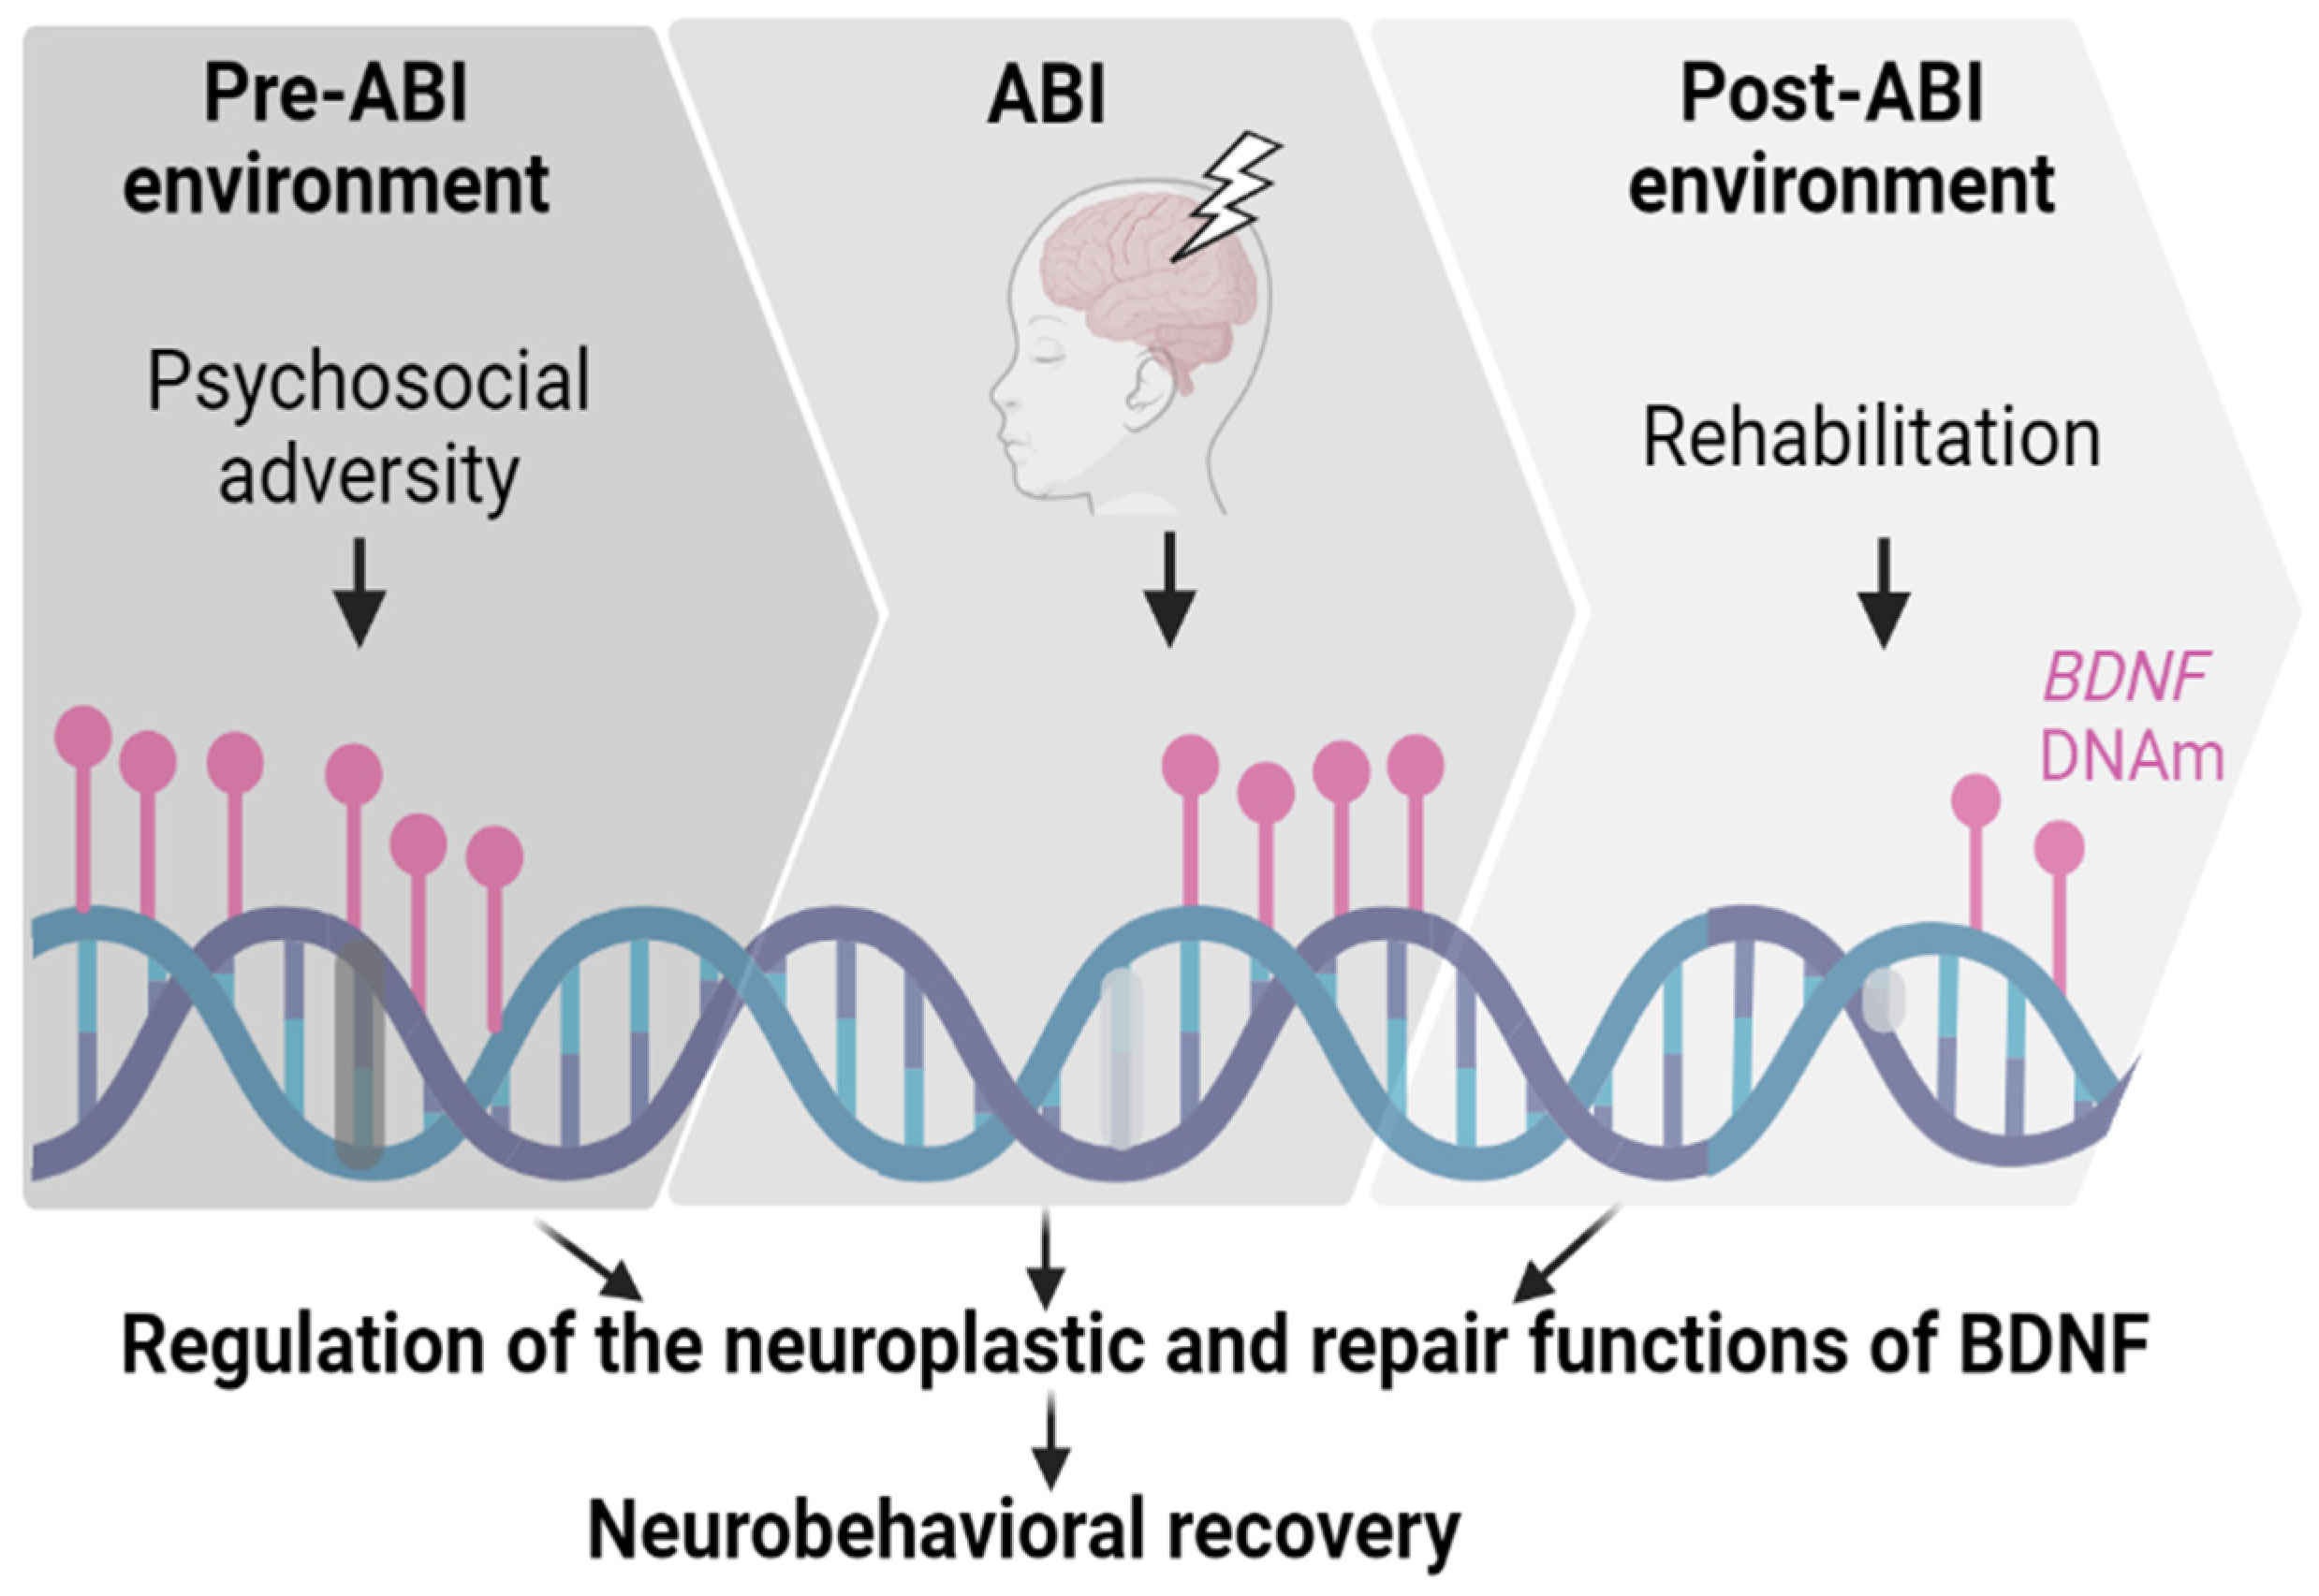
\includegraphics[width=5.20833in,height=\textheight]{eetr.png}
\end{center}

\textbf{E}pigenetic \textbf{E}ffects on Pediatric \textbf{T}raumatic
Brain Injury \textbf{R}ecovery

\section*{Overview}\label{overview-3}
\addcontentsline{toc}{section}{Overview}

\markright{Overview}

EETR is an observational, prospective, longitudinal concurrent cohort
study of children aged 3-18 years with either TBI or orthopedic injury,
recruited from the UPMC Children's Hospital of Pittsburgh. Participants
complete study visits acutely and at 6 and 12 months post-injury.

\section*{Genomic data}\label{genomic-data-1}
\addcontentsline{toc}{section}{Genomic data}

\markright{Genomic data}

\begin{itemize}
\tightlist
\item
  BDNF DNA methylation
\item
  Genome-wide DNA methylation
\item
  BDNF expression data
\end{itemize}

\section*{Eligibility}\label{eligibility-3}
\addcontentsline{toc}{section}{Eligibility}

\markright{Eligibility}

Children aged 3-18 years with either TBI or orthopedic injury and no
history of neurological disorder.

\section*{Study Dates}\label{study-dates-3}
\addcontentsline{toc}{section}{Study Dates}

\markright{Study Dates}

2017 - present

\section*{Ethics}\label{ethics-3}
\addcontentsline{toc}{section}{Ethics}

\markright{Ethics}

The study received ethics approval from the University of Pittsburgh
Institutional Review Board. Participants and their parents provide
informed consent/assent.

\section*{Assessments}\label{assessments-3}
\addcontentsline{toc}{section}{Assessments}

\markright{Assessments}

EETR data collection is conducted at three time points: acute (prior to
hospital discharge) and chronic (at 6 and 12 months post-injury) during
outpatient follow-up visits at CHP. Extensive phenotypic data collection
broadly included hypothesized predictors of neurobehavioral recovery,
neurobehavioral outcomes, and potential confounders/covariates related
to epignetics or neurobehvaioral recovery.

\section*{Team}\label{team-3}
\addcontentsline{toc}{section}{Team}

\markright{Team}

Amery Treble-Barna (PI); Lacey Heinsberg, Dan Weeks, Yvette Conley, Pat
Kochanek, Keith Yeates (Co-Is)

\section*{Funding}\label{funding-3}
\addcontentsline{toc}{section}{Funding}

\markright{Funding}

\begin{itemize}
\tightlist
\item
  \href{https://reporter.nih.gov/search/IEeSkSd_70aDzwz6FxIMDA/project-details/10678647}{K01HD097030}
\item
  \href{https://reporter.nih.gov/search/IEeSkSd_70aDzwz6FxIMDA/project-details/10980135}{R01NS135492}
\end{itemize}

\section*{Related publications}\label{related-publications-3}
\addcontentsline{toc}{section}{Related publications}

\markright{Related publications}

\begin{enumerate}
\def\labelenumi{\arabic{enumi}.}
\item
  Treble-Barna A, Patronick J, Uchani S, Marousis NC, Zigler CK, Fink
  EL, Kochanek PM, Conley YP, Yeates KO. Epigenetic Effects on Pediatric
  Traumatic Brain Injury Recovery (EETR): An Observational, Prospective,
  Longitudinal Concurrent Cohort Study Protocol. Front Neurol. 2020 Jun
  12;11:460. doi: 10.3389/fneur.2020.00460. PMID: 32595586; PMCID:
  PMC7303323.
\item
  Treble-Barna A, Heinsberg LW, Stec Z, Breazeale S, Davis TS, Kesbhat
  AA, Chattopadhyay A, VonVille HM, Ketchum AM, Yeates KO, Kochanek PM,
  Weeks DE, Conley YP. Brain-derived neurotrophic factor (BDNF)
  epigenomic modifications and brain-related phenotypes in humans: A
  systematic review. Neurosci Biobehav Rev.~2023 Apr;147:105078. doi:
  10.1016/j.neubiorev.2023.105078. Epub 2023 Feb 9. PMID: 36764636;
  PMCID: PMC10164361.
\end{enumerate}



\end{document}
